% X（旧 Twitter）に画像 2 枚で投稿するための短い2段組版（A4 2 ページ）。詳しくは main.tex。
\documentclass[a4paper,twocolumn,10pt]{ltjsarticle}
\usepackage[top=8mm,bottom=8mm,left=9mm,right=9mm,columnsep=6mm]{geometry}
\usepackage{amsmath,amssymb}
\usepackage{graphicx}
\usepackage{booktabs}
\usepackage{siunitx}
\usepackage[hidelinks]{hyperref}
\usepackage{enumitem}
\usepackage{caption}
\usepackage{titlesec}
\captionsetup{font=small,skip=2pt}
\setlist{itemsep=0pt,topsep=1pt,parsep=0pt,leftmargin=1.1em}
\titleformat{\section}{\large\bfseries\sffamily}{\thesection}{0.5em}{}
\titlespacing*{\section}{0pt}{5pt plus 1pt}{2pt}
\sisetup{detect-all}
\pagestyle{empty}
\setlength{\parskip}{0pt}
\setlength{\textfloatsep}{6pt plus 2pt minus 2pt}
\setlength{\floatsep}{4pt plus 1pt minus 1pt}
\setlength{\dbltextfloatsep}{6pt plus 2pt minus 2pt}
\newcommand{\figref}[1]{図~\ref{#1}}
\newcommand{\tabref}[1]{表~\ref{#1}}

\begin{document}
\twocolumn[{%
  \begin{center}
    {\LARGE\bfseries 吊り下げボールを壁のすき間に出し入れするクレーン\par}
    \vspace{1mm}
    {\normalsize 軌道最適化 + 時変 LQR による Python での再現と，2 回の独立検証\par}
    \vspace{0.5mm}
    {\normalsize 貝淵蒼馬\par}
  \end{center}
  \vspace{-1mm}
  \noindent\fbox{\parbox{\dimexpr\textwidth-2\fboxsep-2\fboxrule}{\small
    \textbf{要旨}\quad MathWorks のブログ記事\cite{gulley}の「クレーンで吊り荷を振って壁を越えさせる」問題を，MATLAB を使わず Python（CasADi/IPOPT）で再現し，
    \textbf{紐で吊ったボールを 2 枚の壁の間の幅 \SI{42}{cm} のすき間に入れて止める（enter）/ 出して止める（escape）}問題に広げた．
    壁とのすき間 \SI{1.96}{cm} 以上，紐の張力 \SI{1.497}{N} 以上を保ち，力の最大値は短時間版（fast，4 秒）で \SI{20.6}{N}/\SI{22.1}{N}，
    共振を使う長時間版（pump，12 秒）で \SI{12.3}{N}/\SI{13.3}{N}（enter/escape）．
    独立したエージェント群による 2 回の検証で数値は \num{1e-11} 程度まで再現された一方，張力制約の抜けと，力が約 1.7 倍大きい局所解に落ちる問題が見つかり，直した．
    モデル誤差を入れた 1000 回の試行では，escape の成功率 99.5--100\% に対し enter は 86--91\% だった．}}
  \vspace{1.5mm}
  \begin{center}
    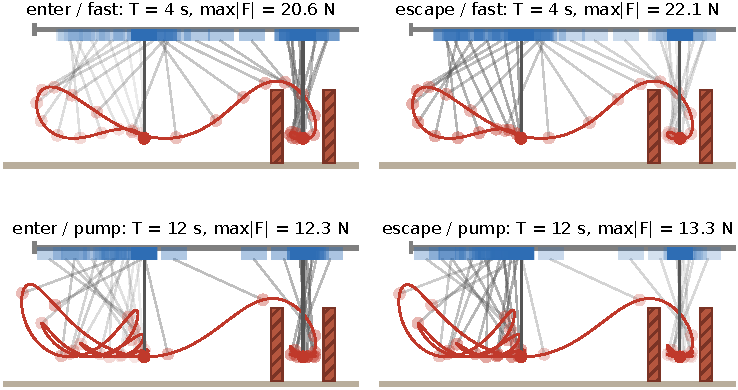
\includegraphics[width=0.86\textwidth]{figs/strobes.pdf}
    \captionof{figure}{4 つの動きのストロボ写真（濃いほど後の時刻）．上段 fast（4 秒），下段 pump（12 秒）．左 enter，右 escape．}
    \label{fig:strobes}
  \end{center}
  \vspace{1mm}
}]

\section{問題}
レール上の台車（\SI{2}{kg}）から長さ \SI{1}{m} の紐で，\SI{1}{kg}・半径 \SI{6}{cm} のボールを吊る．入力は台車を押す水平力 $F$ だけで，
ボールは紐の振れでしか動かせない．床には高さ \SI{0.75}{m}，厚さ \SI{12}{cm} の壁 A，B が立ち，すき間は \SI{42}{cm} しかない．
\begin{itemize}
  \item \textbf{enter}：$x=0$ で静止した状態から，ボールを壁 A の上に振り上げてすき間に入れ，$x=1.63$（すき間の中央）で静止させる．
  \item \textbf{escape}：その逆．すき間で静止した状態から外に出し，$x=0$ で静止させる．
\end{itemize}
制約は，ボールと紐を壁から \SI{2}{cm} 以上離す，紐がたるまない（張力 $\ge \SI{1.5}{N}$），速度 $\le \SI{4}{m/s}$，$|F| \le \SI{40}{N}$，レール端から \SI{3}{cm} 以上．
元記事の剛体の棒ではなく紐で吊るので，張力が正であることも条件になる．

\section{方法}
\textbf{モデル}\quad 台車と振り子の運動方程式（摩擦・減衰込み）．紐の張力は $T_{\mathrm s} = m(g\cos\theta + L\dot\theta^2 - \ddot x\sin\theta)$ で，
$\ddot x$ が $F$ を含むため，力が切り替わる瞬間に張力も跳ぶ．
\textbf{最適化}\quad \SI{20}{ms} ごとに力を一定とする直接多重シューティング法を IPOPT で解く．fast は $\int F^2 dt$，pump は主に $\max|F|$ を最小にする．
壁の制約は非凸なので，低い壁から解き始めて少しずつ高くする．
\textbf{追従と検証}\quad 時変 LQR で追従し（\SI{50}{Hz}），プラントは DOP853（相対誤差 \num{1e-10}）で連続時間のまま積分する．
すき間はボール（円）と紐（線分）で厳密に計算し，張力は力が切り替わる直前の値も含めて確かめる．
\textbf{時間反転}\quad 摩擦がなければ運動方程式は時間反転で変わらないので，enter の逆再生は escape のほぼ実行可能な解になる
（台車の摩擦は $F_r(t) = F(T-t) - 2b\,\dot x(T-t)$ で補正）．実際，enter と escape はほぼ同じ力で済む．

\section{結果}
\begin{table}[t]
  \centering
  \caption{閉ループシミュレーションの結果（モデル誤差なし）．}
  \label{tab:results}
  \small
  \setlength{\tabcolsep}{3pt}
  \begin{tabular}{lcccc}
    \toprule
    & \multicolumn{2}{c}{enter} & \multicolumn{2}{c}{escape} \\
    \cmidrule(lr){2-3}\cmidrule(lr){4-5}
    & fast & pump & fast & pump \\
    \midrule
    時間 [s] & 4 & 12 & 4 & 12 \\
    力の最大値 [N] & 20.6 & 12.3 & 22.1 & 13.3 \\
    ボールと壁 [cm] & 1.96 & 1.96 & 1.96 & 1.96 \\
    紐の張力 [N] & 1.499 & 1.500 & 1.497 & 1.498 \\
    台車の速度 [m/s] & 2.99 & 2.81 & 3.01 & 2.79 \\
    $T$ での誤差 [mm] & \num{1e-5} & \num{7e-7} & \num{5e-7} & \num{1e-6} \\
    \bottomrule
  \end{tabular}
\end{table}
4 つとも壁に当たらず，紐はたるまず，レールと速度の範囲に収まった（\tabref{tab:results}）．
pump は escape ではすき間の中でボールを左右に 3 回ずつ揺らして振り幅を育ててから引き出し，enter では外で振り幅を育ててから入れ，
すき間の中の揺れを押して止める．力の最大値は fast の約 0.6 倍．
ただし元記事の「1/20」には遠い．pump の最大の力はすき間への出入りの瞬間で決まり，$T$ を 30 秒に延ばしても \SI{12.26}{N} までしか下がらない．

\begin{figure*}[t]
  \centering
  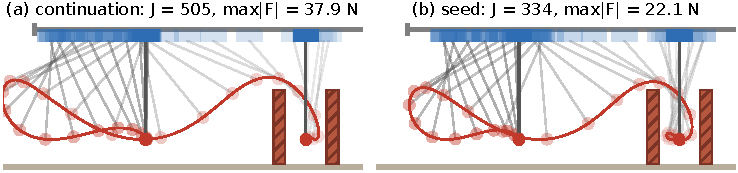
\includegraphics[width=0.95\textwidth]{figs/local_optima_compact.pdf}
  \caption{escape/fast の 2 つの局所解．(a) 低い壁から少しずつ高くして得た解．(b) 細かい時間分割（$N=800$）から得た解．(b) はすき間の中でいったん揺らしてから引き出すので，力の最大値が約 4 割小さい．}
  \label{fig:localopt}
  \vspace{2mm}
  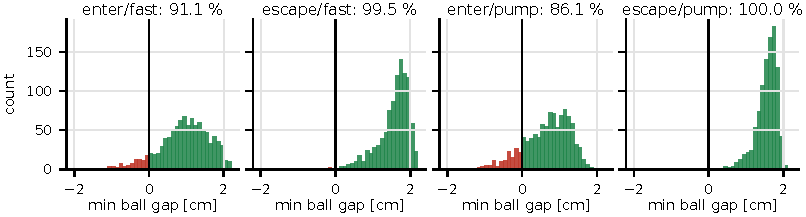
\includegraphics[width=0.95\textwidth]{figs/mc_compact.pdf}
  \caption{モデル誤差を同時に入れた 1000 回の試行（紐の長さ $\pm\SI{1}{\%}$，質量 $\pm\SI{10}{\%}$，摩擦，力の遅れ 0--\SI{10}{ms}，測定ノイズ）でのボールと壁の最小すき間と成功率．赤は壁に接触．}
  \label{fig:mc}
\end{figure*}

\section{局所解：安い工夫では届かない}
最初の実装は escape/fast で \SI{37.9}{N} の解（\figref{fig:localopt}a）を出していたが，\SI{22.1}{N} の解（同 b）がある．
壁の上げ方を変える，すき間で揺らす初期値，長い時間で解いてから縮める，粗い分割の補間はどれも目的関数 $J \approx 500$ の族に落ち，
$J \approx 334$ の族には細かい分割（$N = 600$--1000）で最初から解いたときだけ届いた．
そこで良い解を\textbf{種}として保存し，毎回「ゼロから」「もう一方の動きの時間反転」「種」「種の時間反転・時間伸長」から並列に解いて最良を採る．
約 40 分かけて別の方法でも探したが，\SI{0.5}{\%} 以上良い解はなかった．

\section{2 回の独立検証}
観点ごとにエージェントを並列に走らせ（1 回目 6 観点，2 回目 5 観点），重要な指摘は別のエージェントに反証させた．
独立に導出した運動方程式と \num{3e-14}，別の積分器での再生と \num{1e-11} で一致し，エネルギー収支は \SI{4e-11}{J} で閉じた．
最終結果は独立に作ったシミュレータで \SI{20}{kHz} の格子で再計算し，すべて再現された．見つかって直した主なもの：
\begin{itemize}
  \item 張力の下限を各区間の始点でしか課しておらず，終端では \SI{0.73}{N} まで下がっていた（検証側も見逃していた）→ 始点・中点・終点で課す．
  \item 台車がレール端ぎりぎりを使い，誤差があるとはみ出した → \SI{3}{cm} の余裕と検査．
  \item 力が約 1.7 倍大きい局所解に落ちていた → 種と多点スタート．
\end{itemize}

\section{モデル誤差への強さ}
\begin{table}[t]
  \centering
  \caption{誤差を 1 つずつ入れたとき，最初に失敗する大きさと，\figref{fig:mc} の成功率．（レ）はレール端を越える，（た）は紐がたるむ失敗．ほかは壁への接触．}
  \label{tab:robust}
  \small
  \setlength{\tabcolsep}{2.4pt}
  \begin{tabular}{lcccc}
    \toprule
    & \multicolumn{2}{c}{enter} & \multicolumn{2}{c}{escape} \\
    \cmidrule(lr){2-3}\cmidrule(lr){4-5}
    & fast & pump & fast & pump \\
    \midrule
    紐が長い & +1.8\% & +1.6\% & +3.4\% & +2.9\%（レ） \\
    ボールが軽い & $-13$\% & $-13$\% & なし & なし \\
    クーロン摩擦 & \SI{0.51}{N} & \SI{0.63}{N} & \SI{1.1}{N} & \SI{2.0}{N} \\
    力のむだ時間 & \SI{20}{ms} & \SI{41}{ms} & \SI{35}{ms}（た） & \SI{38}{ms}（た） \\
    \midrule
    成功率 & 91.1\% & 86.1\% & 99.5\% & 100\% \\
    \bottomrule
  \end{tabular}
\end{table}
制御器は名目のモデルで作り，実機側のパラメータだけを変えた（\tabref{tab:robust}，\figref{fig:mc}）．escape は強く，enter は弱い．
計画はどれもボールを壁 A の上面とすき間の両側の面の 3 か所で \SI{2}{cm} まで近づけるが，enter ではすき間の面への接近が追従誤差のたまった後半に来るため，
誤差がどちら向きでも壁に当たる．

\section{まとめと限界}
「動いているように見える」結果でも，独立検証で制約の抜けや局所解が見つかった．残る限界は，enter の弱さ（すき間の面の余裕を大きく取る，ロバスト最適化，積分動作が候補），
空気抵抗・紐の伸び・紐がたるんだ後の運動をモデル化していないこと，解が局所解であること．次は three.js で 3 次元表示にする．

{\footnotesize
\begin{thebibliography}{9}
  \setlength{\itemsep}{0pt}
  \bibitem{gulley} N.~Gulley, ``Simulate in MATLAB, Animate in Blender,'' MATLAB Community Blog, 2026-07-31.
  \bibitem{casadi} J.~A.~E. Andersson et al., \emph{Math. Prog. Comp.}, 11(1):1--36, 2019（CasADi）；
    A.~W\"achter and L.~T. Biegler, \emph{Math. Program.}, 106(1):25--57, 2006（IPOPT）．
\end{thebibliography}}

\end{document}
